\documentclass{article}
\usepackage[T1]{fontenc}
\usepackage{lmodern}
\usepackage{graphicx}
\usepackage{amsmath,amssymb}
\usepackage[a4paper,margin=2cm]{geometry}
\usepackage[absolute,overlay]{textpos}
\setlength{\TPHorizModule}{1mm}
\setlength{\TPVertModule}{1mm}
\usepackage[indonesian]{babel}
\usepackage{hyperref}
\setlength{\emergencystretch}{2em}
% unit: Halaman 32

\begin{document}

% === Halaman 32 (llm) ===

\vspace{114.05mm}

Cover image\vspace{10mm}
Stego-image

\vspace{114.05mm}

% deskripsi: Gambar asli (cover image) yang menampilkan seekor kucing Scottish Fold yang sedang dielus.
% bbox normalisasi: [0.1940, 0.0900, 0.5880, 0.4740]
\begin{textblock*}{82.74mm}(40.74mm,26.73mm)
\noindent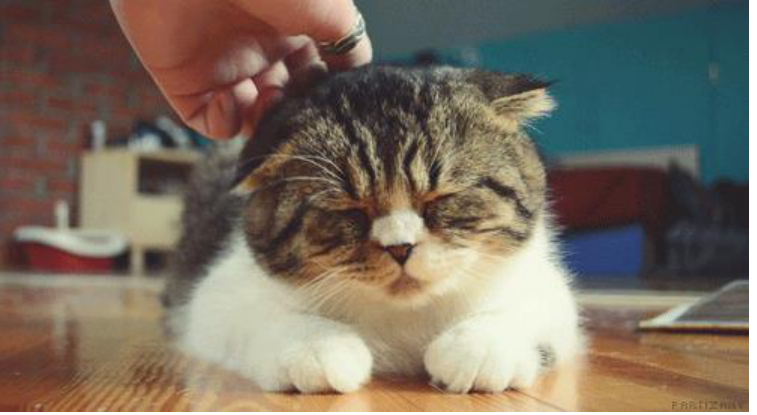
\includegraphics[width=82.74mm,height=114.05mm]{../../images/llm/page_032_img_01.png}%
\end{textblock*}

% deskripsi: Gambar stego (stego-image) yang secara visual tampak identik dengan cover image namun mengandung data tersembunyi.
% bbox normalisasi: [0.4380, 0.5260, 0.8320, 0.9100]
\begin{textblock*}{82.74mm}(91.98mm,156.22mm)
\noindent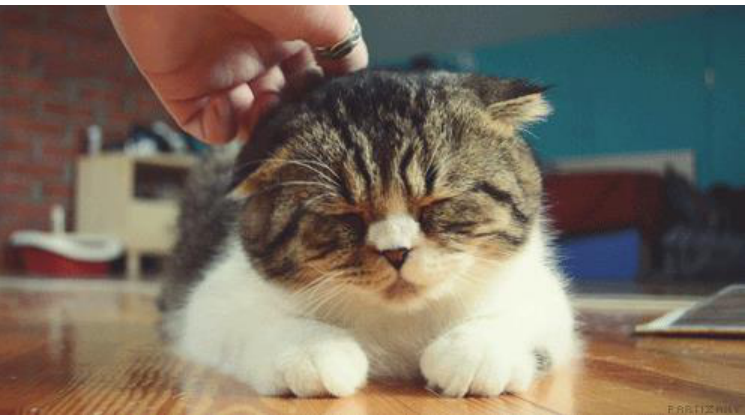
\includegraphics[width=82.74mm,height=114.05mm]{../../images/llm/page_032_img_02.png}%
\end{textblock*}

\end{document}
